% !TeX root = ../main.tex

\chapter{多租户性能隔离的云闪存系统设计}
\label{chap:design}

本章介绍本研究提出的多租户性能隔离的云闪存系统设计。
\autoref{sec:design-overview}是对该系统各组件的功能和每一租户获取、访问资源的流程概述。
\autoref{sec:design-array}介绍了本系统通过将SSD的访问时间窗口划分为独立的纯读和纯写窗口,并将多个这样的SSD组成无读写干扰的SSD阵列。
\autoref{sec:design-allocation}介绍了本系统通过静态数据分布和动态IO调度来减轻SSD上多租户间的读写干扰。

\section{系统总述}
\label{sec:design-overview}

如\autoref{fig:design-overview}所示,本系统主要由控制器、客户端和存储单元组成。
其中,控制器负责管理存储单元,并根据租户的需求用尽可能经济的方式为其分配存储空间。
为了避免存储空间的碎片化,控制器以\textit{块}为单位管理存储空间,例如10GB为一个块。
客户端位于租户的虚拟机上,它负责与控制器沟通,并代替租户进行存储资源访问。
存储单元可能是一块SSD或多块SSD组成的存储阵列(~\autoref{sec:design-array}),不同的存储单元可以提供不同的SLA保证,也有不同的开销。
例如,一个存储单元可能用3块SSD的冗余提供99\%分位数的尾延迟保证,而另一个存储单元可能仅能提供90\%的保证,但只需要花费一块SSD。

\begin{figure}[h]
  \centering
  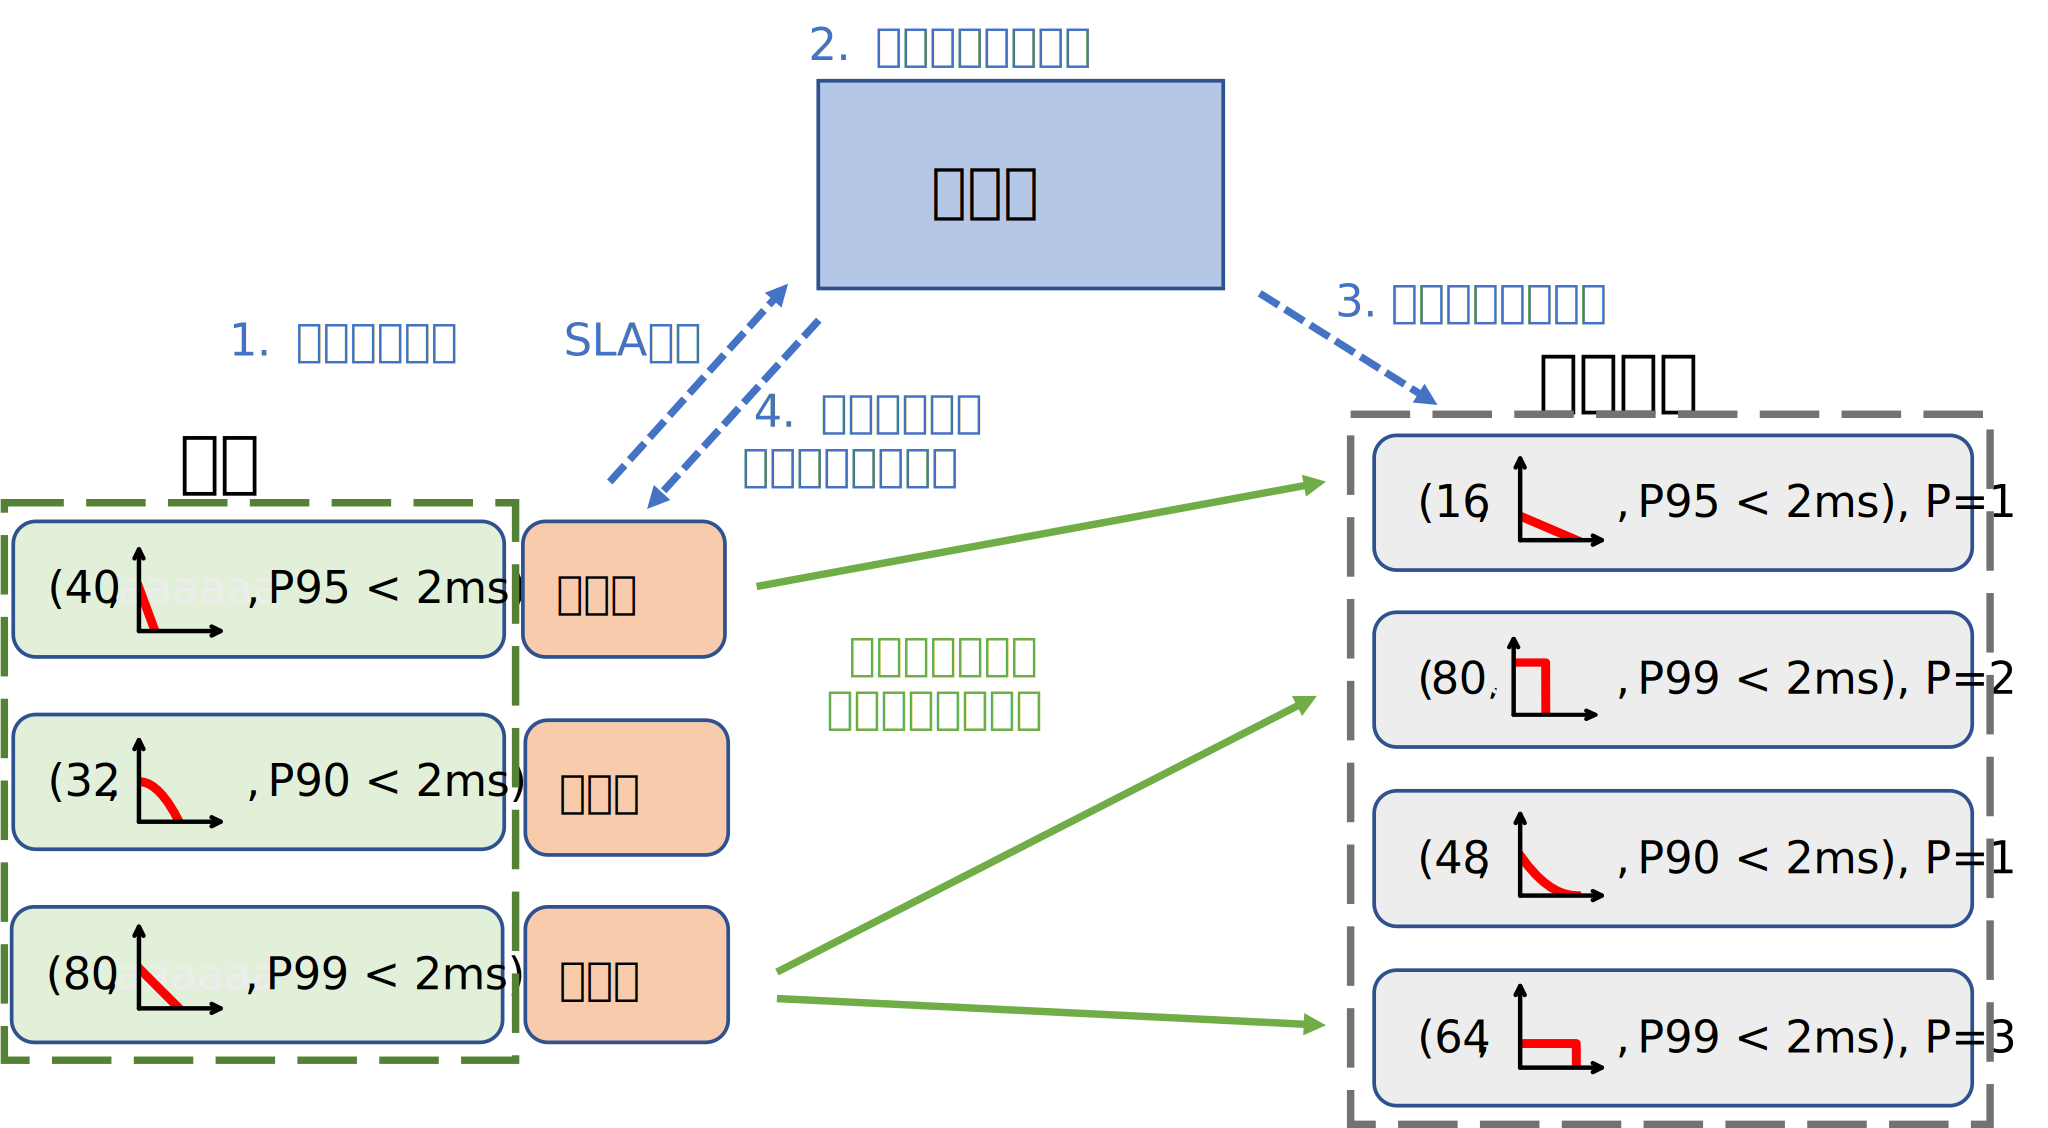
\includegraphics[width=0.8\textwidth]{thesis-design.pdf}
  \caption{
      本系统的总体概述。
      租户和存储单元以(存储数据块数,SLA曲线,尾延迟要求)这个三元组来描述,存储单元还有开销P。
      图中蓝色虚线标示的是新租户进入本系统时的控制路径,
      绿色实线标示的是系统中的租户访问存储单元时的数据路径。
      }
  \label{fig:design-overview}
\end{figure}

在本系统中,每个租户的资源需求和每个存储单元能提供的服务能力均以$(C, S, T)$这一三元组定义。
其中,$C$表示存储空间(Capacity),例如40个块;
$S$表示SLA曲线(SLA Curve);
$T$表示尾延迟要求(Tail latency),例如延迟的99\%分位数小于2ms($P99 < 2ms$)。 
由于存储单元的异构性,每个存储单元还有自身的开销$P$。

本系统的控制路径由\autoref{fig:design-overview}中的蓝色虚线表示。
当一个用户加入系统时,他首先通过客户端将自己的资源需求以以上三元组的形式发送给控制器。
控制器以块为单位管理用户的存储需求。
由于每个用户的各个块之间是条带化的\cite{patterson1988case},因此SLA曲线也可以平均分配到每个块上。
根据\autoref{sec:design-allocation}中提出的启发式数据分布算法,控制器优先将尽可能多的块放于已启用的存储单元上。
若已启用的存储单元不足以容纳用户的资源需求,则根据存储单元的开销$P$选择最经济的方式存放剩余的存储需求。
此时若有需要,控制器还需要负责建立新的存储单元(\autoref{sec:design-array})。
在控制器确定该用户的数据分布后,他将该租户的存储空间中每个块与对应的存储单元及存储单元中该块的起始地址的映射发送给租户服务器上的客户端。

\autoref{fig:design-overview}中的绿色实线表示的是本系统的数据路径。
当租户需要访问其所拥有的存储空间时,客户端根据该映射选择合适的存储单元,并将租户存储空间内的逻辑地址转换为存储单元的逻辑地址,从而代替租户访问存储单元。
客户端根据租户的SLA曲线对租户的读写速率进行限制,从而保证租户得到自身的SLA保证。
该客户端可以实现在软件的块设备层~\cite{linuxblock},也可以在智能网卡通过硬件实现~\cite{bluefield}。

\section{无读写干扰的SSD阵列}
\label{sec:design-array}

云存储系统的某些租户可能具有苛刻的尾延迟要求。
然而,如\autoref{fig:bg-wr-interfere}所示,SSD上程度很小的读写干扰就可能使其尾延迟难以达到租户的要求。
因此,本节提出无读写干扰的SSD阵列,它可以在读写吞吐都很大的情况下避免读写干扰的发生。
本系统利用上述SSD阵列作为一种存储单元,来提供高度的尾延迟保证。

\subsection{分离的读写时间窗口}
\label{sec:design-array-isorw}

\begin{figure}[h]
  \centering
  \includegraphics[width=0.95\textwidth]{thesis-wr-mix.pdf}
  \caption{
        Samsung PM963上,读吞吐为150KIOPS,写吞吐为30KIOPS时,读请求的异常延迟在出现的时间间隔上没有明确的规律,而且持续时长也不确定。
      }
  \label{fig:design-wr-mix}
\end{figure}

本小节给出在单一SSD上避免读写干扰的方法,该方法基于如下对读写干扰产生的根本原因的分析。
\autoref{fig:design-wr-mix}采样了在读吞吐为150KIOPS,写吞吐为30KIOPS时,200ms内Samsung PM963上读请求的延迟情况。
可以看出,异常延迟的总次数并不多,因此它们仅影响了读请求的尾延迟。
然而,由于这些异常延迟的出现没有明确的规律且持续时长难以预测(\autoref{chap:background}),所以我们难以找到避免异常延迟的方法。

针对该问题,本研究提出,避免对不规律的异常延迟进行困难且准确度低的预测,转而控制这些异常延迟的发生时间和时长。
本研究作出的观察是,尽管异常延迟的出现是难以预测的,但它们均是由读写干扰问题造成的。
也就是说,如果避免发送写请求,则读请求基本不会出现异常的延迟。

因此,本研究提出\textit{分离的读写时间窗口},即将对SSD的访问时间划分为独立的纯读和纯写时间窗口。
如\autoref{fig:design-iso-wr}所示,读写窗口交替出现,在任何一个时刻,SSD上均只有读或写中的一种操作。
在读窗口中,所有写请求被缓存于缓冲区中,SSD上只进行读操作,从而保证不会有异常延迟出现;
在写窗口中,SSD不再接受读操作,之前被缓存的写请求被批量发送。
由于批量发送可以充分利用SSD内部的并行度,因此可以充分利用SSD的写带宽。

\begin{figure}[h]
  \centering
  \includegraphics[width=0.8\textwidth]{thesis-iso-wr.pdf}
  \caption{
        分离的读写时间窗口在单块SSD上的工作流程。
        在读窗口中,所有写请求被缓存于缓冲区中,从而保证读请求的尾延迟;
        在写窗口中,之前被缓存的写请求被批量发送,充分利用SSD的写带宽。
      }
  \label{fig:design-iso-wr}
\end{figure}

\autoref{fig:design-wr-isolated}描述了分离的读写时间窗口对SSD的读延迟分布的影响。
通过将写操作在写窗口中批量发送,所有可能出现异常读延迟的情况都被限制在了写窗口中。
通过避免在写窗口中发送读请求,租户可以在在读窗口中获得稳定的读延迟。

\begin{figure}[h]
  \centering
  \includegraphics[width=0.95\textwidth]{thesis-wr-isolated.pdf}
  \caption{
        同样的请求模式下,启用分离的读写窗口时,不仅异常延迟的数量减少了,而且所有的异常延迟均被控制在写窗口中出现,
        读窗口内可以得到稳定的尾延迟。
      }
  \label{fig:design-wr-isolated}
\end{figure}

\subsection{读写窗口协调的冗余磁盘阵列}
\label{sec:design-array-composition}

尽管上一节提出的分离的读写窗口可以使读请求在读窗口中得到不受干扰的读延迟,但它不能在写窗口中接受读请求。
对于现代的在线事务处理服务来讲,对于存储服务的读访问往往处于其关键路径上。
因此,单块SSD的写窗口时间如果过长,会导致其读访问排队延迟过大,使得分离的读写窗口得不偿失。

遗憾的是,在实践中,写窗口的时间不能很短。
% 由\autoref{fig:design-wr-window-size}可见,即使写窗口已经结束,下一个读窗口起始处的一些读请求仍会出现异常延迟。
这是由于写操作触发的垃圾回收、缓冲区刷新等SSD内部维护操作是异步进行的。
在写操作完成后,这些操作仍在进行,从而使得下一个读窗口起始处的一些读请求出现异常延迟。
因此,SSD上读写窗口的时间不能过短,否则过于频繁的窗口切换会影响大量读请求的延迟,从而大大影响总体的尾延迟。

针对这一问题,本研究提出使用\textit{具有冗余的SSD阵列}来掩盖SSD的写窗口。
由于具有冗余的SSD阵列(例如RAID~\cite{patterson1988case}或纠删码~\cite{huang2012erasure})具有从若干台SSD的故障中恢复的能力,所以可以将处于写窗口中的SSD视为“故障”。
通过协调各个SSD上的读写窗口,可以保证同时处于写窗口中的SSD数量不多于阵列的恢复能力。
当有面向处于写窗口中的SSD数据的读请求时,可以利用其它SSD中的数据恢复该SSD中的数据。
由于其它SSD均处于读窗口中,具有良好的访问延迟,因此对处于写窗口中SSD数据的恢复也具有良好的延迟。
此外,由于未被完全写入的写数据总在缓冲区中存有一份拷贝,各个SSD上的数据一致性也得到了保证。

例如,在\autoref{fig:design-ssd-array}中,利用3块SSD组成了一个RAID-5磁盘阵列。
通过协调三台SSD交替进入写窗口,该阵列保证任一时间都只有一台SSD不可读。
由于RAID-5具有从一块磁盘故障中恢复的能力,因此对所有数据的读都有较低的尾延迟。
比如当SSD \#1处于写窗口时,对其中数据的读,可以通过先读取SSD \#2和SSD \#3的相应数据,之后进行异或运算实现。

\begin{figure}[h]
  \centering
  \includegraphics[width=0.8\textwidth]{thesis-ssd-array.pdf}
  \caption{
        用RAID-5组成读写窗口协调的冗余SSD阵列。
        通过协调各个SSD上的读写窗口,可以保证同时最多有一台SSD处于写窗口。
        由于RAID-5可以从一块磁盘的故障中恢复,所以所有数据总可以被以无干扰的读延迟访问。
      }
  \label{fig:design-ssd-array}
\end{figure}

\section{基于SLA曲线的资源分配}
\label{sec:design-allocation}

通过构建无读写干扰的SSD阵列,本系统可以保证具有严格尾延迟要求的租户的服务质量。
然而,如\autoref{chap:background}所说,云系统中租户的尾延迟要求是多样的,并非所有租户都需要严格无读写干扰的存储服务。
况且,\autoref{sec:design-array}中搭建的SSD阵列利用了冗余,成本较高。
因此,一个自然的问题就是,当一个租户进入系统时,如何为其进行资源分配,可以使系统整体的开销尽可能少?
此处的资源分配,即指静态的数据分布,也指运行时的带宽分配。

本章提出一个基于\autoref{chap:intro}提出的SLA曲线的多租户数据分布算法。
本章首先根据数据分布问题的特点定义了SLA曲线的加法、减法和除法操作。
随后,本章参考装箱问题~\cite{wiki:Bin-packing}中的最佳适应(Best Fit)算法,并运用针对SLA曲线提出的适应性函数,提出了一个启发式的多租户数据分布算法。
之后,本章又设计了一个基于时间片和限速(Rate Limiting)的IO调度器,确保运行时每个租户都遵守其SLA曲线,从而满足租户的服务质量。

\subsection{SLA曲线及其运算}
\label{sec:design-allocation-sla-arithmetic}

本节中,将SLA曲线表示为最大读吞吐作为写吞吐的函数。
具体来讲,对于SLA曲线$A$,$A[w] = r$表示在写吞吐为$w$下,在满足尾延迟要求的情况下能达到的最大读吞吐为$r$。

\begin{figure}[h]
  \centering
  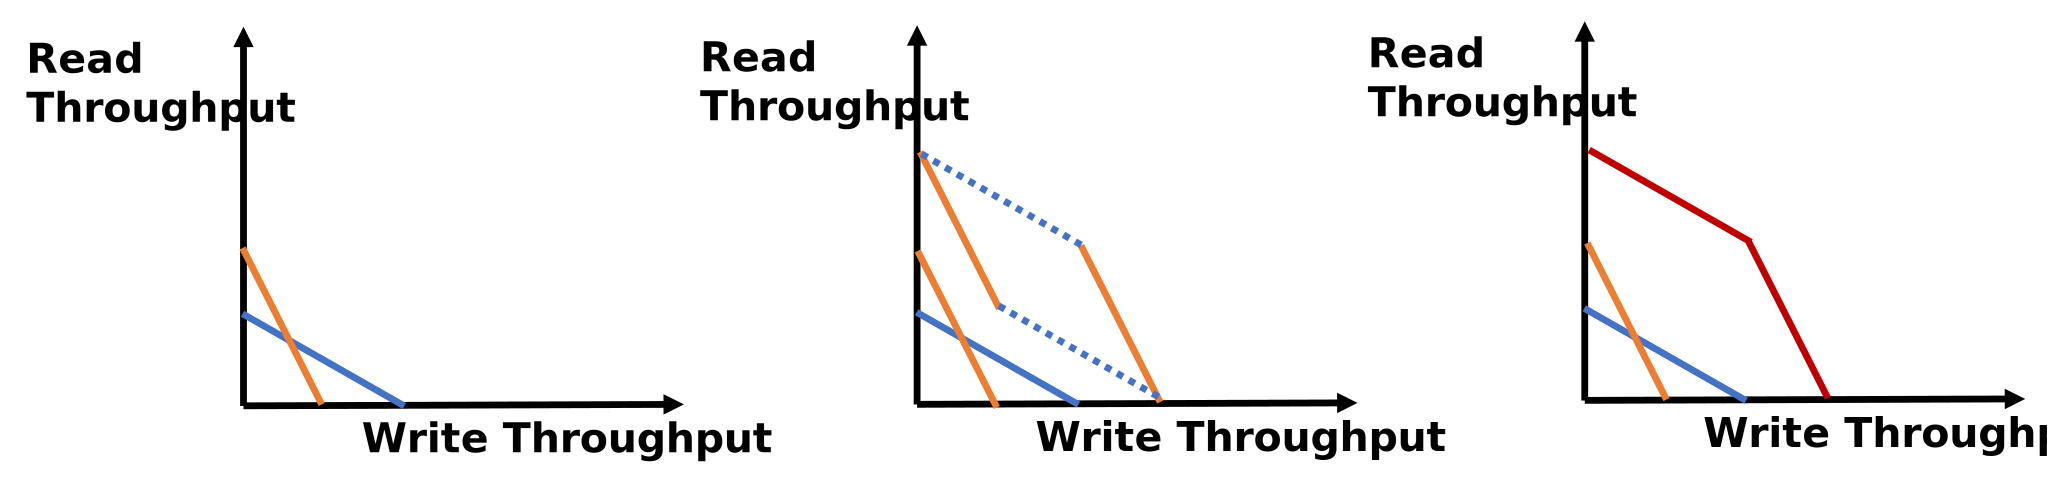
\includegraphics[width=1.0\textwidth]{thesis-sla-add.pdf}
  \caption{
        两个SLA曲线A、B之和是能够同时满足A和B的SLA要求的最小曲线。
        图中橙色和蓝色曲线为两个租户的SLA曲线,红色为两者之和。
      }
  \label{fig:design-sla-add}
\end{figure}

当两个租户同时运行在一台SSD上时,总体的读和写吞吐是两者吞吐的叠加。
由于SLA曲线代表了用户需求的最低保证,因此,他们总体的SLA曲线应代表两者所有可能的吞吐组合的最大值。
为了方便描述多个租户共同的SLA,本节定义SLA曲线的加法和数乘如下:

\begin{definition}
  \textit{SLA曲线的加法和数乘}

  若A和B均为SLA曲线,则定义$C=A+B$为:
  \begin{equation}
    C[w] = \max_{0 \le i \le w} (A[i] + B[w - i])
  \end{equation}

  根据加法的定义,定义SLA曲线的\textbf{数乘}为$k * A$为$k$个SLA曲线$A$的累加。

\end{definition}

SLA曲线加法如\autoref{fig:design-sla-add}所示。

除此之外,一个存储单元是否能满足一个租户的SLA需求,是由租户的SLA曲线是否在存储单元的SLA曲线覆盖的范围内确定的。
为了描述这种关系,本节定义SLA曲线的\textit{包含}如下:

\begin{definition}
  \textit{SLA曲线的包含}

  若A和B均为SLA曲线,则$A\preceq B$(A\textbf{包含}在B中),当且仅当$\forall w$,若$A[r] > 0$,则有$A[w] \le B[w]$。
\end{definition}

\begin{figure}[h]
  \centering
  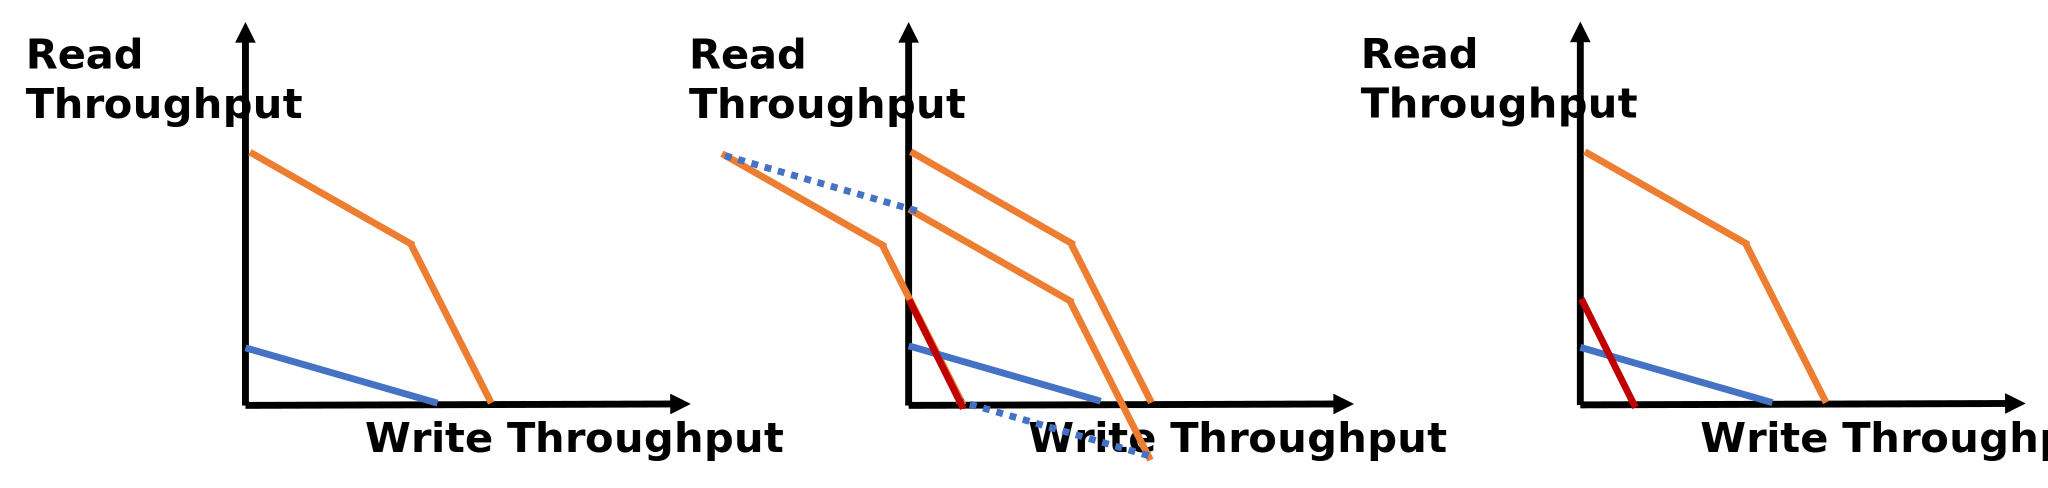
\includegraphics[width=1.0\textwidth]{thesis-sla-subtract.pdf}
  \caption{
        两个SLA曲线A、B之差是在满足B的SLA要求的情况下,A还能满足的最大SLA曲线。
      }
  \label{fig:design-sla-subtract}
\end{figure}

有了加法和包含的定义后,本节继续定义SLA曲线的减法。
减法的使用场景为,当一个租户使用一个存储单元时,存储单元剩余的可用存储带宽会相应下降。
其剩余的存储带宽应当为在满足该租户的SLA曲线情况下,还能容纳的最大带宽。
因此,这两个SLA曲线的差应该代表他们所有吞吐组合之差的最小值。
具体来讲,SLA曲线的差定义如下:

\begin{definition}
  \textit{SLA曲线的减法}

  若A和B均为SLA曲线,且$B \preceq A$,则定义$C=A-B$为:
  \begin{equation}
    C[w] = \min_{i} (A[i] - B[i - r])
  \end{equation}
\end{definition}

根据如上减法的定义,本文继续定义SLA曲线的带余除法如下:

\begin{definition}
  \textit{SLA曲线的带余除法}

  若A和B均为SLA曲线,且$B \preceq A$,则定义A与B的商和模为:
  \begin{equation}
    \begin{split}
      A / B & = \max k \in \mathbb{Z}^{+} s.t. k * B \preceq A \\
      A \% B & = A - (A / B) * B
    \end{split}
  \end{equation}
\end{definition}


\subsection{基于SLA曲线的多租户数据分布算法}
\label{sec:design-allocation-algo}

在多租户的云闪存系统中,多个租户如何在众多资源中选择最合适的分布,使得他们的需求被满足,且整体开销最低,可以被建模为经典的\textit{装箱问题}~\cite{wiki:Bin-packing}。
装箱问题的背景是,将一系列大小不同的一维物体装入若干个大小一致的箱子中,使得使用的总箱子数尽可能少。

装箱问题的一个常见在线算法是\textit{最佳适应}(Best Fit)。
该算法是一个启发式贪心算法,可以概括为:
每当一个新物体加入时,将其放入可以容纳它的剩余空间最小(最适应)的箱子中;
若没有箱子可以容纳它,则启用一个新的箱子来存放它。

本系统参考最佳适应算法进行数据分布,但是基于SLA曲线的多租户数据分布问题与典型的装箱问题相比,主要有以下区别:

\begin{enumerate}
  \item 租户的资源需求和存储单元的服务能力(\textit{物体})以SLA曲线表示,无法明确比较大小。因此,为租户选择“最适应”的存储单元是困难的。
  \item 不同的存储单元(\textit{箱子})有不同的服务能力,而且有不同的开销。因此,需要启用新的箱子时,需要选择启用哪种存储单元。
  \item 本系统的用户需求是可分的,可以通过条带化等方法将用户的数据块分散在不同的存储单元中,进一步提高利用率。
\end{enumerate}

针对以上问题,本系统提出的贪心算法(~\autoref{algo:tenant-allocation})对最佳适应算法做出了改进。

\IncMargin{1em}
\begin{algorithm}[h]
  \SetAlgoLined
  \SetKwData{Suitable}{unitChoices}\SetKwData{SortedUnits}{sortedUnits}
  \SetKwData{Request}{request}\SetKwData{OpenUnits}{openUnits}\SetKwData{UnitTypes}{unitTypes}
  \SetKwData{U}{u}
  \SetKwData{UT}{ut}
  \SetKwData{BestType}{bestType}
  \SetKwData{BestCost}{bestCost}
  \SetKwData{CostForRequest}{costForRequest}
  \SetKwFunction{Filter}{Filter}
  \SetKwFunction{Fitness}{Fitness}
  \KwData{用户请求\Request,已启用的存储单元列表\OpenUnits,可选的存储单元类型\UnitTypes,均以$(C, S, T)$的形式表示,每个存储单元类型有开销$P$}
  \BlankLine

  \tcp{将\Request 中的数据块尽可能存入已开启的存储单元中}
  \Suitable$\leftarrow$ \Filter{\OpenUnits, \Request.T} \;% $\leftarrow$ \;% \Filter{$open\_units$, $request\.T$}\;
  Sort \Suitable by \Fitness \; \label{algo:fitness-sort}

  \ForEach{ \U in \Suitable }{
    尽可能多地将\Request 中的数据块存放于\U 中 \;
    \lIf(\tcp*[h]{\Request 中所有的数据块都已分配完毕}){\Request $.C$ == 0}{
      \Return{}
    }
  }

  \tcp{需要启用新的存储单元,贪心地选择用最小开销容纳剩余的数据块}
  
  \BestCost $\leftarrow$ $+\infty$

  \ForEach{ \UT in \UnitTypes }{
    \CostForRequest $\leftarrow$ 容纳\Request 所需的\UT 个数$\times$\UT .P \;
    \If{\CostForRequest $<$ \BestCost}{
      \BestType $\leftarrow$ \UT \;
      \BestCost $\leftarrow$ \CostForRequest \;
    }
  }

  启用\BestType 类型存储单元来存放\Request 中的数据块 \;

  \caption{租户进入系统时的数据分布算法}
  \label{algo:tenant-allocation}
\end{algorithm}
\DecMargin{1em}

首先,针对SLA曲线的“最适应”和数据可分的问题,本算法参考向量背包问题~\cite{panigrahy2011heuristics},提出使用\textit{Fitness}函数为所有存储单元排序(\autoref{algo:fitness-sort}),
之后按照Fitness函数确定的适应性顺序,将用户需求中尽可能多的数据块存入对应的存储单元中。
本节提出以下可能的Fitness函数,由于篇幅限制,下文未对它们进行比较,但是在实践中它们的效果基本一致。

\begin{itemize}
  \item 存储单元和它最多可容纳的租户数据块SLA曲线与X、Y轴围成的的\textbf{面积比}。这个量度不考虑形状,只选择大小最接近的。
  \item 存储单元和它最多可容纳的租户数据块SLA曲线的\textbf{点积}。\citet{panigrahy2011heuristics,gabay2016vector}指出,使用向量的点积可以找出“形状”最匹配且大小最接近的向量,SLA曲线也同理。
  \item 存储单元和它最多可容纳的租户数据块SLA曲线的\textbf{$L_2$范数}。与点积同理,$L_2$范数也倾向于选择最接近用户SLA曲线的存储单元。
\end{itemize}

除此之外,针对存储单元的异构问题,本算法采用贪心的方式选择对当前租户需求来说开销最小的存储单元。
具体来讲,针对每种存储单元,本算法依次计算利用其存储用户需求所需要的开销,并从中选择开销最小的存储单元。

\subsection{基于SLA曲线的运行时IO调度}

上一小节提出的数据分布算法在租户进入系统时的数据分布环节确保了各个租户分得的资源不会超过存储单元最大的承载量。
但是租户不会一直按其被分配的资源发送IO请求,因此运行时的IO调度器需要能够确保租户始终运行在自身的SLA曲线内。

本系统的IO调度器设计是基于时间片和限速(rate limiting)的,与一般的限速不同,基于SLA曲线的IO调度对租户的每一个写吞吐,设置一个对应的读吞吐上限。
每个时间片中,每个租户被记录下已经发送的读吞吐和写吞吐。
当租户发送读请求时,IO调度器根据SLA曲线查询当前写吞吐对应的最大读吞吐,并依据其对读请求进行限速;
当租户发送写请求时,IO调度器根据SLA曲线查询发送该写请求后当前读吞吐是否将超过了新的写吞吐对应的最大读吞吐,并据此对写请求进行限速。
此外,在保证整个存储单元的读写吞吐不超过存储单元的SLA曲线的前提下,IO调度器可以允许租户短暂超过它的SLA曲线。
当多个租户都超过其SLA曲线时,请求按Round Robin方式实现公平调度。

本系统的IO调度器的另一个设计要点在于其多队列、多线程的设计,利用一个独立的线程进行请求调度,避免线程之间的锁操作影响整体的性能。
这一部分将在\autoref{chap:impl}详细介绍。